\documentclass{beamer}
\usepackage[utf8]{inputenc}

\usetheme{Madrid}
\usecolortheme{default}
\usepackage{amsmath,amssymb,amsfonts,amsthm}
\usepackage{txfonts}
\usepackage{tkz-euclide}
\usepackage{listings}
\usepackage{adjustbox}
\usepackage{array}
\usepackage{tabularx}
\usepackage{gvv}
\usepackage{lmodern}
\usepackage{circuitikz}
\usepackage{tikz}
\usepackage{graphicx}

\setbeamertemplate{page number in head/foot}[totalframenumber]

\usepackage{tcolorbox}
\tcbuselibrary{minted,breakable,xparse,skins}



\definecolor{bg}{gray}{0.95}
\DeclareTCBListing{mintedbox}{O{}m!O{}}{%
  breakable=true,
  listing engine=minted,
  listing only,
  minted language=#2,
  minted style=default,
  minted options={%
    linenos,
    gobble=0,
    breaklines=true,
    breakafter=,,
    fontsize=\small,
    numbersep=8pt,
    #1},
  boxsep=0pt,
  left skip=0pt,
  right skip=0pt,
  left=25pt,
  right=0pt,
  top=3pt,
  bottom=3pt,
  arc=5pt,
  leftrule=0pt,
  rightrule=0pt,
  bottomrule=2pt,

  colback=bg,
  colframe=orange!70,
  enhanced,
  overlay={%
    \begin{tcbclipinterior}
    \fill[orange!20!white] (frame.south west) rectangle ([xshift=20pt]frame.north west);
    \end{tcbclipinterior}},
  #3,
}
\lstset{
    language=C,
    basicstyle=\ttfamily\small,
    keywordstyle=\color{blue},
    stringstyle=\color{orange},
    commentstyle=\color{green!60!black},
    numbers=left,
    numberstyle=\tiny\color{gray},
    breaklines=true,
    showstringspaces=false,
}
%------------------------------------------------------------
%This block of code defines the information to appear in the
%Title page
\title %optional
{2.8.9}
\date{september 2025}
%\subtitle{A short story}

\author % (optional)
{J.NAVYASRI- EE25BTECH11028}

\begin{document}

\frame{\titlepage}
\begin{frame}{Question}
Let $\vec{a}, \vec{b}, \vec{c}$ be three vectors such that 
$|\vec{a}|=3,\; |\vec{b}|=4,\; |\vec{c}|=5$, and each one of them is perpendicular to the sum of the other two. 
Find $|\vec{a}+\vec{b}+\vec{c}|$.
\end{frame}


\begin{frame}{Solution:}
From the identity:
\begin{equation} \label{eq1}
\mathbf{a}^\top(\mathbf{b} + \mathbf{c}) = 0,
\end{equation}
we expand:
\begin{equation} \label{eq2}
\mathbf{a}^\top \mathbf{b} + \mathbf{a}^\top \mathbf{c} = 0.
\end{equation}

Similarly, from the symmetry of dot products:
\begin{align}
\mathbf{b}^\top \mathbf{c} + \mathbf{b}^\top \mathbf{a} &= 0, \label{eq3} \\
\mathbf{c}^\top \mathbf{a} + \mathbf{c}^\top \mathbf{b} &= 0. \label{eq4}
\end{align}

Let
\begin{equation} \label{eq5}
x = \mathbf{a}^\top \mathbf{b}, \quad y = \mathbf{b}^\top \mathbf{c}, \quad z = \mathbf{c}^\top \mathbf{a}.
\end{equation}
\end{frame}

\begin{frame}{Solution:}
Then equations (2), (3), and (4) become:
\begin{align}
x + z &= 0, \label{eq6} \\
x + y &= 0, \label{eq7} \\
y + z &= 0. \label{eq8}
\end{align}

\bigskip

\noindent
\textbf{Matrix Form:}  
Equations (6), (8) can be written compactly as
\[
\myvec{
1 & 0 & 1 \\
1 & 1 & 0 \\
0 & 1 & 1
}
\myvec{
x \\ y \\ z
}
=
\myvec{
0 \\ 0 \\ 0
}.
\]

\end{frame}

\begin{frame}{Solution:}
Therefore:
\begin{equation} \label{eq9}
x = y = z = 0,
\end{equation}
so $\mathbf{a}, \mathbf{b}, \mathbf{c}$ are \textbf{pairwise orthogonal}.

\bigskip

The \textbf{Gram matrix} of $ (\mathbf{a}, \mathbf{b}, \mathbf{c}) $ is:
\begin{equation} \label{eq10}
G =
\myvec{
\mathbf{a}^\top \mathbf{a} & \mathbf{a}^\top \mathbf{b} & \mathbf{a}^\top \mathbf{c} \\
\mathbf{b}^\top \mathbf{a} & \mathbf{b}^\top \mathbf{b} & \mathbf{b}^\top \mathbf{c} \\
\mathbf{c}^\top \mathbf{a} & \mathbf{c}^\top \mathbf{b} & \mathbf{c}^\top \mathbf{c}
}
=
\myvec{
\|\mathbf{a}\|^2 & 0 & 0 \\
0 & \|\mathbf{b}\|^2 & 0 \\
0 & 0 & \|\mathbf{c}\|^2
}
=
\myvec{
9 & 0 & 0 \\
0 & 16 & 0 \\
0 & 0 & 25
}.
\end{equation}

Let
\[
\mathbf{u} = \myvec{1 \\ 1 \\ 1}.
\]
\end{frame}

\begin{frame}{Solution:}
Then
\begin{equation} \label{eq11}
\|\mathbf{a} + \mathbf{b} + \mathbf{c}\|^2 = (\mathbf{a} + \mathbf{b} + \mathbf{c})^\top (\mathbf{a} + \mathbf{b} + \mathbf{c}) = \mathbf{u}^\top G \mathbf{u}.
\end{equation}

Now compute:
\begin{align}
\mathbf{u}^\top G \mathbf{u} 
&= \myvec{1 & 1 & 1}
\myvec{
9 & 0 & 0 \\
0 & 16 & 0 \\
0 & 0 & 25
}
\myvec{1 \\ 1 \\ 1} \nonumber \\
&= 9 + 16 + 25 = 50. \label{eq12}
\end{align}

Therefore:
\begin{equation} \label{eq13}
\|\mathbf{a} + \mathbf{b} + \mathbf{c}\| = \sqrt{50} = 5\sqrt{2}.
\end{equation}

\bigskip

\textbf{Final Answer:}
\[
\boxed{5\sqrt{2}}
\]

\end{frame}

\begin{frame}[fragile]
    \frametitle{Python Code}
    \begin{lstlisting}
import numpy as np
import matplotlib.pyplot as plt

# Define mutually perpendicular vectors
a = np.array([3, 0, 0])
b = np.array([0, 4, 0])
c = np.array([0, 0, 5])
s = a + b + c   # resultant (3,4,5)

fig = plt.figure(figsize=(8, 6))
ax = fig.add_subplot(111, projection='3d')
\end{lstlisting}
\end{frame}


\begin{frame}[fragile]
    \frametitle{Python Code}
    \begin{lstlisting}
# Plot main vectors
ax.quiver(0, 0, 0, *a, color='r', linewidth=2,
          arrow_length_ratio=0.08, normalize=False, label='a (3)')
ax.quiver(0, 0, 0, *b, color='g', linewidth=2,
          arrow_length_ratio=0.08, normalize=False, label='b (4)')
ax.quiver(0, 0, 0, *c, color='b', linewidth=2,
          arrow_length_ratio=0.08, normalize=False, label='c (5)')

# Plot resultant
ax.quiver(0, 0, 0, *s, color='m', linewidth=2,
          arrow_length_ratio=0.05, normalize=False,
          label='a+b+c')
\end{lstlisting}
\end{frame}


\begin{frame}[fragile]
    \frametitle{Python Code}
    \begin{lstlisting}
# Axis limits
ax.set_xlim(0, 8)
ax.set_ylim(0, 8)
ax.set_zlim(0, 8)

# Axis labels
ax.set_xlabel("X-axis")
ax.set_ylabel("Y-axis")
ax.set_zlabel("Z-axis")
ax.set_title("Mutually Perpendicular Vectors and their Resultant")

ax.legend()
plt.show()

\end{lstlisting}
\end{frame}

\begin{frame}[fragile]
\frametitle{C Code}
\begin{lstlisting}
#include <stdio.h>
#include <math.h>

int main() {
    // Given magnitudes
    int a = 3, b = 4, c = 5;
    // Since a, b, c are mutually perpendicular (proved in solution),
    // |a + b + c|^2 = |a|^2 + |b|^2 + |c|^2
    int sum_sq = a*a + b*b + c*c;

    double magnitude = sqrt(sum_sq);

    // Print result
    printf("The magnitude |a + b + c| = %.2f\n", magnitude);

    return 0;
}
\end{lstlisting}

\end{frame}


\begin{frame}{Plot-Using by Python}
    \centering
    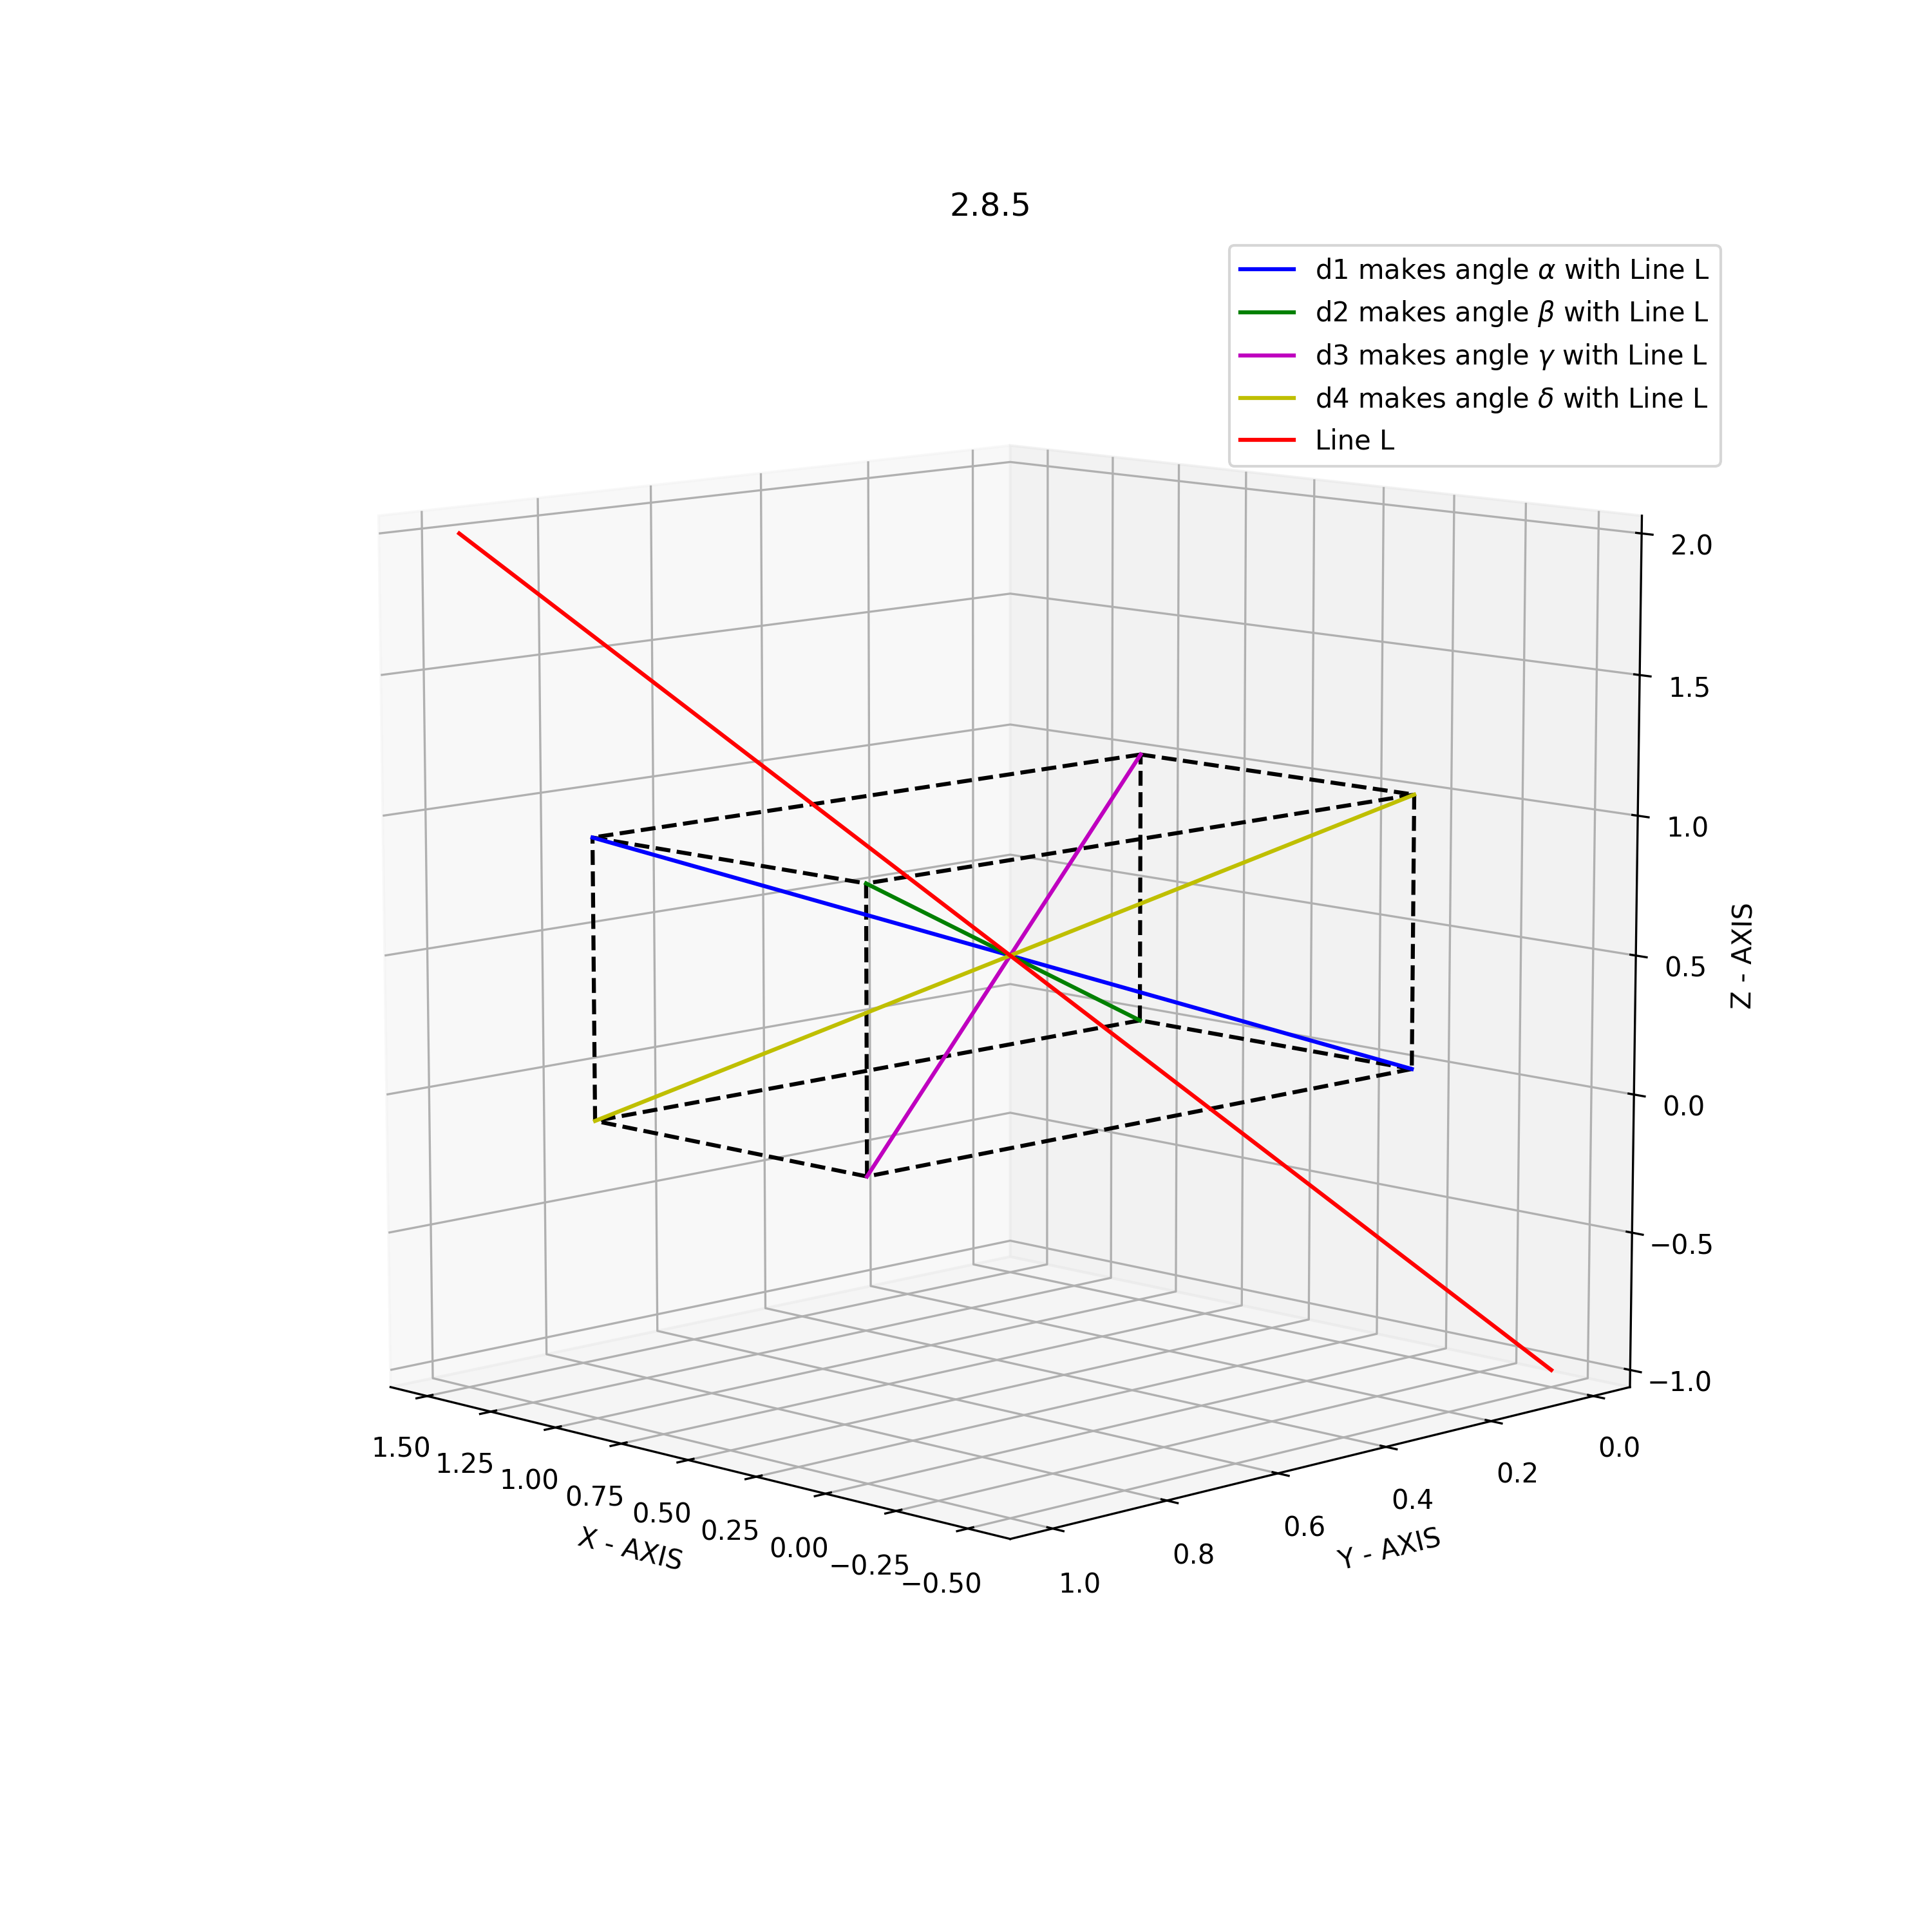
\includegraphics[width=\columnwidth, height=0.8\textheight, keepaspectratio]{fig4.png}     
\end{frame}


\begin{frame}[fragile]
\frametitle{Python and C Code}

\begin{lstlisting}
import ctypes
import numpy as np
import matplotlib.pyplot as plt

# Load the compiled C library
lib = ctypes.CDLL("./vector_calc.so")   # use "vector_calc.dll" on Windows

# Call the C function
lib.vector_magnitude.restype = ctypes.c_double
magnitude = lib.vector_magnitude()
print("Result from C code |a+b+c| =", magnitude)
\end{lstlisting}

\end{frame}
\begin{frame}[fragile]
\frametitle{Python and C Code}

\begin{lstlisting}
# ---- Plotting in Python ----
a = np.array([3, 0, 0])
b = np.array([0, 4, 0])
c = np.array([0, 0, 5])
resultant = a + b + c

fig = plt.figure(figsize=(8, 6))
ax = fig.add_subplot(111, projection="3d")

# plot vectors
origin = np.array([0, 0, 0])
ax.quiver(*origin, *a, color='r', label='a (3)')
ax.quiver(*origin, *b, color='g', label='b (4)')
ax.quiver(*origin, *c, color='b', label='c (5)')
ax.quiver(*origin, *resultant, color='m', label='a+b+c')
\end{lstlisting}

\end{frame}
\begin{frame}[fragile]
\frametitle{Python and C Code}

\begin{lstlisting}
ax.set_xlim([0, 8])
ax.set_ylim([0, 8])
ax.set_zlim([0, 8])

ax.set_xlabel("X axis")
ax.set_ylabel("Y axis")
ax.set_zlabel("Z axis")
ax.set_title("C code calculation + Python plot")

ax.legend()
plt.show()
\end{lstlisting}

\end{frame}

\begin{frame}{Plot-Using by both C and Python}
    \centering
    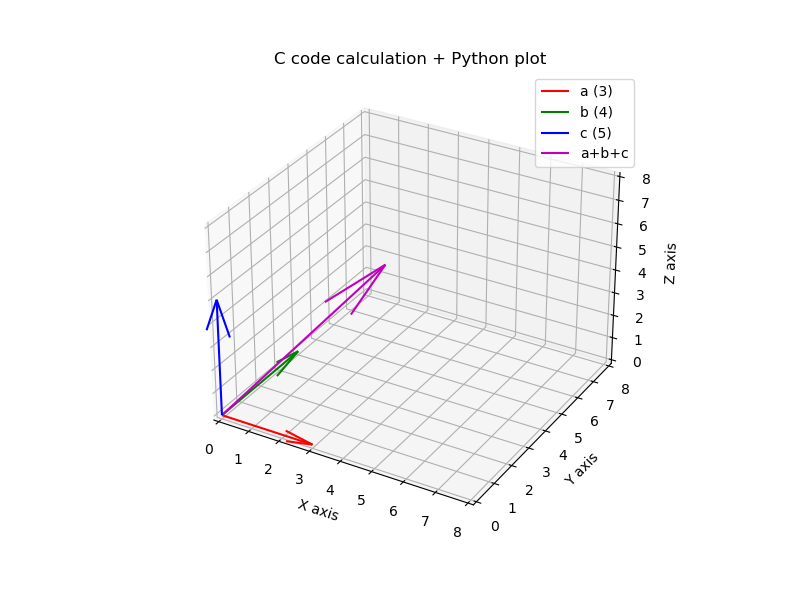
\includegraphics[width=\columnwidth, height=0.8\textheight, keepaspectratio]{figs/fig4.1.png}     
\end{frame}

\end{document}


